\documentclass[ 12pt ]{article}

\usepackage{amsmath}
\usepackage{amssymb}
\usepackage{cancel}
\usepackage{tikz}

\begin{document}

% title page
\title{Homework 1}
\author{Landon Fox}
\date{February 6, 2020}

\begin{flushleft}
Landon Fox \\
CS 326 \\
Section 1001 \\
February 6, 2020
\end{flushleft}
\begin{center}
Homework 1
\end{center}

% problem 1
\section{}
Programming Language: C

% problem 1a
\subsection{}
The declaration of a variable with the leading character being a digit.

% problem 1b
\subsection{}
A function call without a semicolon at the end of the statement.

% problem 1c
\subsection{}
Indexing an array using a float.

% problem 1d
\subsection{}
Indexing an array with an index greater than the last element; out of bounds error.
\newpage

% problem 2
\section{}

% problem 2a
\subsection{}
\begin{flalign}
R=ab(\epsilon|(a|b)^*b)a
\end{flalign}

% problem 2b
\subsection{}
\begin{flalign}
R=(0|1|2|3|4|5|6|7|8|9)^*(0|5)
\end{flalign}

% problem 2c
\subsection{}
\begin{flalign}
R=(aa)^*
\end{flalign}

% problem 3
\section{}

% problem 3a
\subsection{}
\begin{flalign}
S_1 &\rightarrow aS_2ba \\
S_2 &\rightarrow \epsilon|bS_3 \\
S_3 &\rightarrow \epsilon|aS_3|bS_3
\end{flalign}

% problem 3b
\subsection{}
\begin{flalign}
S_1 &\rightarrow \epsilon|aaS_1S_2 \\
S_2 &\rightarrow \epsilon|bbS_2
\end{flalign}

% problem 3c
\subsection{}
\begin{flalign}
S &\rightarrow \epsilon|(S)|[S]|\{S\}|SS
\end{flalign}

% problem 4
\section{}
Language L is defined by the grammar:
\begin{flalign}
P &\rightarrow [B,P]|B \\
B &\rightarrow D|(P) \\
D &\rightarrow x|y|z
\end{flalign}

% problem 4a
\subsection{}
\begin{flalign}
&z \epsilon L \\
&P \rightarrow B \rightarrow D \rightarrow z
\end{flalign}

% problem 4b
\subsection{}
\begin{flalign}
&(x) \epsilon L \\
&P \rightarrow B \rightarrow (P) \rightarrow (B) \rightarrow (D) \rightarrow (x)
\end{flalign}

% problem 4c
\subsection{}
\begin{flalign}
&[y] \cancel{\epsilon} L \\
\end{flalign}

% problem 4d
\subsection{}
\begin{flalign}
&([x,y]) \epsilon L \\
&P \rightarrow B \rightarrow (P) \rightarrow ([B,P]) \rightarrow ([D,P]) \\
&\rightarrow ([x,P]) \rightarrow ([x,B]) \rightarrow ([x,P]) \rightarrow ([x,B]) \\
&\rightarrow ([x,D]) \rightarrow ([x,y])
\end{flalign}

% problem 4e
\subsection{}
\begin{flalign}
&[(x),y] \epsilon L \\
&P \rightarrow [B,P] \rightarrow [(P),P] \rightarrow [(B),P] \rightarrow [(D),P] \\
&\rightarrow [(x),P] \rightarrow [(x),B] \rightarrow [(x),D] \rightarrow [(x),y]
\end{flalign}

% problem 5a
\section{}
\begin{flalign}
AssignStmt &\rightarrow Var=E \\
Var &\rightarrow id|id[Index] \\
Index &\rightarrow E \\
E &\rightarrow Var|nr|E+E|E-E|E*E|E/E|(E)
\end{flalign}

% problem 5ai
\subsection{}
\begin{flalign}
a[2]=b+1
\end{flalign}
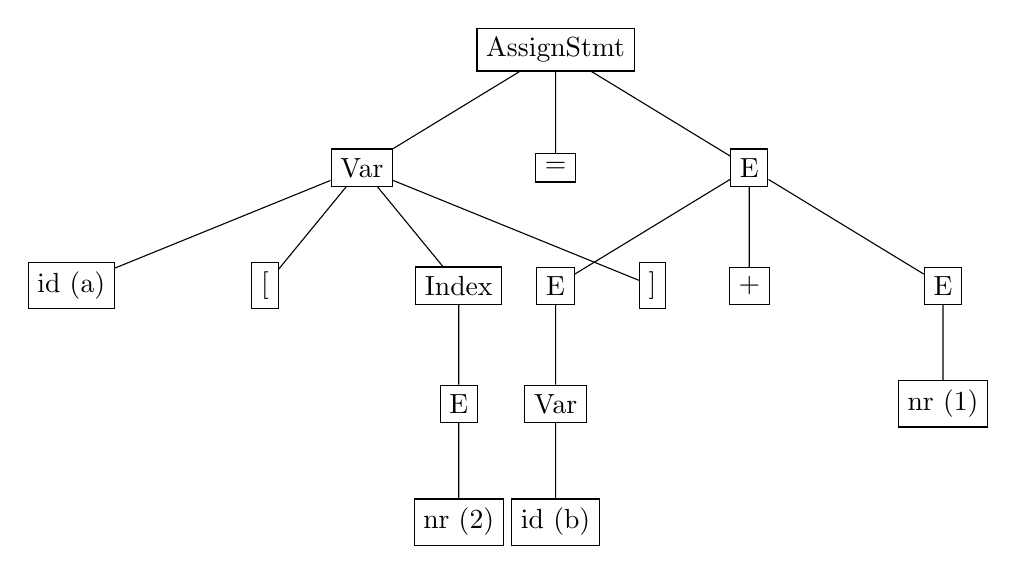
\begin{tikzpicture}[sibling distance=7em,
  every node/.style = {shape=rectangle,
    draw, align=center,
    top color=white, bottom color=white!20}]]
  \node {AssignStmt}
    child { node {Var}
      child { node {id (a)} }
	  child { node {[} }
	  child { node {Index}
	  	child { node {E}
	  		child { node {nr (2)} } } }
	  child { node {]} } }
    child { node {=} }
    child { node {E}
      child { node {E} 
      	child { node {Var}
      		child { node {id (b)} } } }
      child { node {+} }
      child { node {E} 
      	child { node {nr (1)} } } };
\end{tikzpicture}
\newpage

% problem 5aii
\subsection{}
\begin{flalign}
x=v[k-3]
\end{flalign}
\begin{tikzpicture}[sibling distance=7em,
  every node/.style = {shape=rectangle,
    draw, align=center,
    top color=white, bottom color=white!20}]]
  \node {AssignStmt}
    child { node {Var}
      child { node {id (x)} } }
    child { node {=} }
    child { node {E}
      	child { node {Var}
      		  child { node {id (v)} }
			  child { node {[} }
			  child { node {Index}
			  	child { node {E}
			  		child { node {E} 
			  			child { node {Var} 
			  				child { node {id (k)} } } }
			      	child { node {-} }
			      	child { node {E} 
			      		child { node {nr (3)} } } } }
			  child { node {]} } } };
\end{tikzpicture}
\newpage

% problem 5b
\subsection{}
\begin{flalign}
AssignStmt &\rightarrow Var=E \\
Var &\rightarrow id|id[Index] \\
Index &\rightarrow E,E|E \\
E &\rightarrow Var|nr|E+E|E-E|E*E|E/E|(E)
\end{flalign}

% problem 6
\section{}
\begin{flalign}
R=\epsilon|b|bR|aRa
\end{flalign}

\end{document}
